\documentclass{beamer}
\usetheme{metropolis}           % Use metropolis theme

\usepackage{tikz}
\usepackage{smartdiagram}
\usepackage[utf8]{inputenc}
\usepackage[spanish]{babel}

\usepackage{smartdiagram}
\usepackage{verbatim}
\usepackage{svg}
\usepackage{graphicx}
\usepackage{color}
\definecolor{lightgray}{rgb}{0.95, 0.95, 0.95}
\definecolor{darkgray}{rgb}{0.4, 0.4, 0.4}
%\definecolor{purple}{rgb}{0.65, 0.12, 0.82}
\definecolor{editorGray}{rgb}{0.95, 0.95, 0.95}
\definecolor{editorOcher}{rgb}{1, 0.5, 0} % #FF7F00 -> rgb(239, 169, 0)
\definecolor{editorGreen}{rgb}{0, 0.5, 0} % #007C00 -> rgb(0, 124, 0)
\definecolor{orange}{rgb}{1,0.45,0.13}		
\definecolor{olive}{rgb}{0.17,0.59,0.20}
\definecolor{brown}{rgb}{0.69,0.31,0.31}
\definecolor{purple}{rgb}{0.38,0.18,0.81}
\definecolor{lightblue}{rgb}{0.1,0.57,0.7}
\definecolor{lightred}{rgb}{1,0.4,0.5}
\usepackage{upquote}
\usepackage{listings}
\lstset{language=html,
	basicstyle=\footnotesize\ttfamily,
	keywordstyle=\footnotesize\color{blue}\ttfamily,
}
% CSS
\lstdefinelanguage{CSS}{
	keywords={color,background-image:,margin,padding,font,weight,display,position,top,left,right,bottom,list,style,border,size,white,space,min,width, transition:, transform:, transition-property, transition-duration, transition-timing-function},	
	sensitive=true,
	morecomment=[l]{//},
	morecomment=[s]{/*}{*/},
	morestring=[b]',
	morestring=[b]",
	alsoletter={:},
	alsodigit={-}
}

% JavaScript
\lstdefinelanguage{JavaScript}{
	basicstyle=\scriptsize\ttfamily,
	morekeywords={typeof, new, true, false, catch, function, return, null, catch, switch, var, if, in, while, do, else, case, break, \$scope},
	morecomment=[s]{/*}{*/},
	morecomment=[l]//,
	morestring=[b]",
	morestring=[b]'
}

\lstdefinelanguage{HTML5}{
	basicstyle=\scriptsize\ttfamily,
	language=html,
	sensitive=true,	
	alsoletter={<>=-},	
	morecomment=[s]{<!-}{-->},
	tag=[s],
	otherkeywords={
		% General
		>,
		% Standard tags
		<!DOCTYPE,
		</html, <html, <head, <title, </title, <style, </style, <link, </head, <meta, />,
		% body
		</body, <body,
		% Divs
		</div, <div, </div>, 
		% Paragraphs
		</p, <p, </p>,
		% scripts
		</script, <script,
		% More tags...
		<canvas, /canvas>, <svg, <rect, <animateTransform, </rect>, </svg>, <video, <source, <iframe, </iframe>, </video>, <image, </image>, <header, </header, <article, </article, <input, </input, <h1, </h1
	},
	ndkeywords={
		% General
		=,
		% HTML attributes
		charset=, src=, id=, width=, height=, style=, type=, rel=, href=,
		% SVG attributes
		fill=, attributeName=, begin=, dur=, from=, to=, poster=, controls=, x=, y=, repeatCount=, xlink:href=,
		% properties
		margin:, padding:, background-image:, border:, top:, left:, position:, width:, height:, margin-top:, margin-bottom:, font-size:, line-height:,
		% CSS3 properties
		transform:, -moz-transform:, -webkit-transform:,
		animation:, -webkit-animation:,
		transition:,  transition-duration:, transition-property:, transition-timing-function:,
		%Angular
		ng-body=, ng-model=, ng-bind=, ng-controller=, ng-click=
	}
}
\metroset{background=dark} 


%\usebackgroundtemplate%
%{%
%	
\includegraphics[width=\paperwidth]{Images/fondo}%
%}

\title{Testing para Java EE}
\author{Víctor Orozco}
\institute{Nabenik}
\date{\today}

\begin{document}

\frame{\titlepage}


\begin{frame}{Víctor Orozco}
\begin{columns}[T] % contents are top vertically aligned
	\begin{column}[T]{5cm} % each column can also be its own environment
		\begin{itemize}
			\item Developer (JVM/Open Source Advocate)
			\item JUG Leader
			\item Consultor independiente
			\item Profesor universitario
			\item \href{https://twitter.com/tuxtor}{@tuxtor}
			\item \href{http://vorozco.com}{http://vorozco.com}
			\item \href{http://tuxtor.shekalug.org}{http://tuxtor.shekalug.org} 
		\end{itemize}
	\end{column}
	\begin{column}[T]{5cm} % alternative top-align that's better for graphics
		\begin{figure}
			\centering
			
\includegraphics[width=0.6\linewidth]{Images/logos}
		\end{figure}
		
	\end{column}
\end{columns}
\end{frame}


\begin{frame}{Pruebas}
\begin{figure}
	\centering
	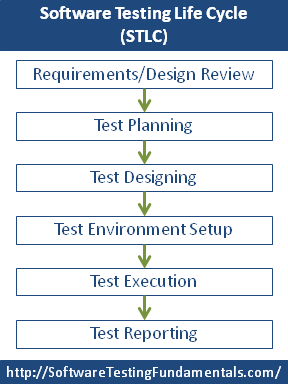
\includegraphics[width=0.4\linewidth]{Images/lifecycle}
\end{figure}
\end{frame}


\begin{frame}{Unit Testing - Tipos}
\begin{columns}[T]
\begin{column}[T]{6cm}
	\begin{itemize}
		\item Funcionamiento de cada unidad
		\item Estructurado: Programa, función, procedimiento
		\item POO: Clase y derivados (servicio, endpoint)
		\item Frameworks, drivers, stubs, mocks
		\item Developers
		\item Tip: Probar lo que tiene impacto
	\end{itemize}
\end{column}
\begin{column}[T]{4cm} % alternative top-align that's better for graphics
	\begin{figure}
		\centering
		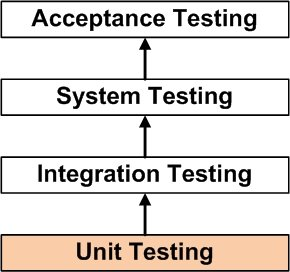
\includegraphics[width=0.8\linewidth]{Images/unittesting}
	\end{figure}
\end{column}
\end{columns}
\end{frame}

\begin{frame}{Integration Testing - Tipos}
\begin{columns}[T]
\begin{column}[T]{6cm}
\begin{itemize}
	\item Unidades combinadas
	\item Interfaces e integraciones
	\item Sistemas externos
	\item Frameworks, White Box, Black Box
	\item Developers y testers
	\item Tip: Documentar integraciones
\end{itemize}
\end{column}
\begin{column}[T]{4cm} % alternative top-align that's better for graphics
\begin{figure}
	\centering
	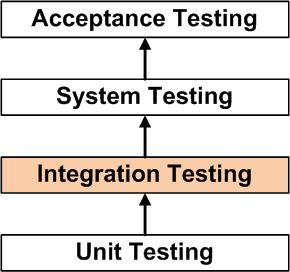
\includegraphics[width=0.8\linewidth]{Images/integrationtesting}
\end{figure}

\end{column}
\end{columns}
\end{frame}

\begin{frame}{System Testing - Tipos}
\begin{columns}[T]
\begin{column}[T]{6cm}
\begin{itemize}
\item Sistema vs. requerimientos
\item Black Box
\item Testers
\item Tip: Requerimientos actualizados
\end{itemize}
\end{column}
\begin{column}[T]{4cm} % alternative top-align that's better for graphics
\begin{figure}
\centering
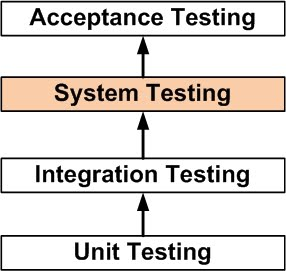
\includegraphics[width=0.8\linewidth]{Images/systemtesting}
\end{figure}
\end{column}
\end{columns}
\end{frame}

\begin{frame}{Acceptance Testing - Tipos}
\begin{columns}[T]
\begin{column}[T]{6cm}
\begin{itemize}
\item Requerimientos vs. necesidades reales
\item Ad-hoc
\item Pruebas internas: Alpha, Testers
\item Pruebas externas: Beta, Usuarios y clientes
\end{itemize}
\end{column}
\begin{column}[T]{4cm} % alternative top-align that's better for graphics
\begin{figure}
\centering
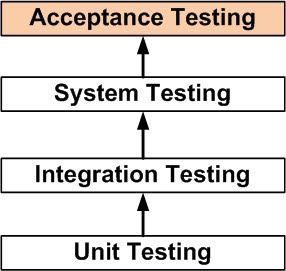
\includegraphics[width=0.8\linewidth]{Images/acceptancetesting}
\end{figure}
\end{column}
\end{columns}
\end{frame}


\begin{frame}{Black box - Técnicas}
\begin{columns}[T]
\begin{column}[T]{4cm}
\begin{itemize}
\item Integration
\item System
\item Acceptance
\end{itemize}
\end{column}
\begin{column}[T]{6cm} % alternative top-align that's better for graphics
\begin{figure}
\centering
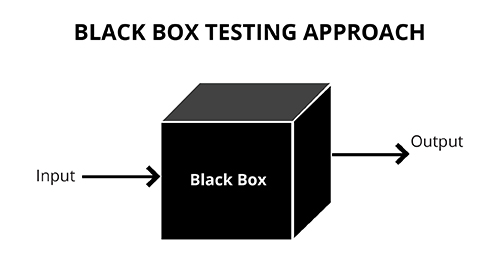
\includegraphics[width=\linewidth]{Images/blackboxtesting.jpg}
\end{figure}
\end{column}
\end{columns}
\end{frame}

\begin{frame}{White box - Técnicas}
\begin{columns}[T]
\begin{column}[T]{4cm}
\begin{itemize}
\item Unit
\item Integration
\item System

\end{itemize}
\end{column}
\begin{column}[T]{6cm} % alternative top-align that's better for graphics
\begin{figure}
\centering
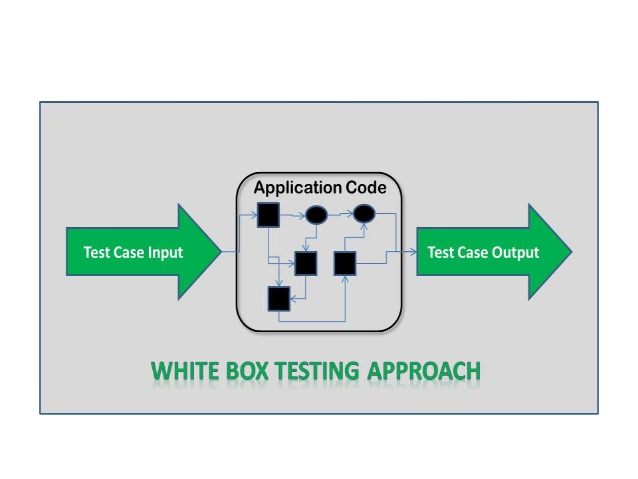
\includegraphics[width=\linewidth]{Images/whiteboxtesting.jpg}
\end{figure}
\end{column}
\end{columns}
\end{frame}


\begin{frame}{Ad hoc - Técnicas}
\begin{columns}[T]
\begin{column}[T]{4cm}
\begin{itemize}
\item Acceptance
\item Monkey Testing
\end{itemize}
\end{column}
\begin{column}[T]{6cm} % alternative top-align that's better for graphics
\begin{figure}
\centering
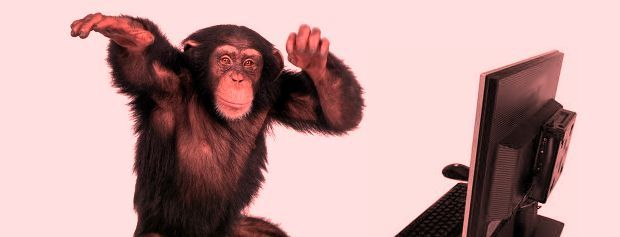
\includegraphics[width=\linewidth]{Images/adhoctesting.jpg}
\end{figure}
\end{column}
\end{columns}
\end{frame}


\begin{frame}{TDD - Técnicas}
\begin{columns}[T]
\begin{column}[T]{4cm}
\begin{itemize}
\item Unit
\item Integration
\end{itemize}
\end{column}
\begin{column}[T]{6cm} % alternative top-align that's better for graphics
\begin{figure}
\centering
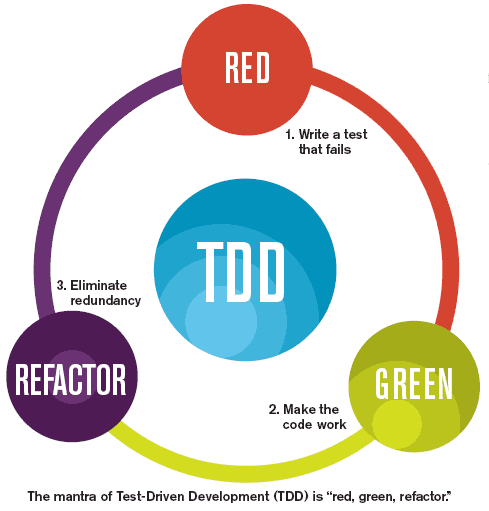
\includegraphics[width=0.9\linewidth]{Images/tdd}
\end{figure}
\end{column}
\end{columns}
\end{frame}

\section{Unit testing}

\begin{frame}{Unit Testing - Java}
\begin{columns}[T]
	\begin{column}[T]{6cm}
		\begin{itemize}
			\item JUnit, TestNG
			\item Mockito, JMock, JMockit
			\item Arquillian (parcialmente)
		\end{itemize}
	\end{column}
	\begin{column}[T]{4cm} % alternative top-align that's better for graphics
		\begin{figure}
			\centering
			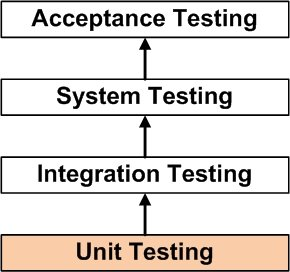
\includegraphics[width=0.8\linewidth]{Images/unittesting}
		\end{figure}
	\end{column}
\end{columns}
\end{frame}


\section{JUnit 4}

\begin{frame}{JUnit 4}
	\begin{itemize}
		\item Primera prueba
		\item @Before @After
		\item Asserts
		\item @BeforeClass @AfterClass
		\item Pruebas parametrizadas
		\item Suites
	\end{itemize}
\end{frame}

\begin{frame}[containsverbatim]{JUnit - BeforeClass - AfterClass}
Se ejecuta una vez por \textit{testing class}, como primera acción
\begin{lstlisting}[language=Java]
@BeforeClass
public static void setUpClass() {
	System.out.println("First on every class");
}
\end{lstlisting}

Se ejecuta una vez por \textit{testing class}, como ultima acción
\begin{lstlisting}[language=Java]
@AfterClass
public static void tearDownClass() {
	System.out.println("Last on every class");
}
\end{lstlisting}
\end{frame}

\begin{frame}[containsverbatim]{JUnit - Before - After}
Se ejecuta una vez por \textit{@Test}, como primera acción
\begin{lstlisting}[language=Java]
@Before
public void testSetup(){
	System.out.println("First on every test");
}
\end{lstlisting}

Se ejecuta una vez por \textit{@Test}, como ultima acción
\begin{lstlisting}[language=Java]
@After
public void destroyTest(){
	System.out.println("Test ending");
}
\end{lstlisting}
\end{frame}

\begin{frame}[containsverbatim]{JUnit - Test}
Ejecuta una prueba completa a partir de la comprobación de \textit{asserts}
\begin{lstlisting}[language=Java]
@Test
public void testProduct(){
	System.out.println("Product");
	assertEquals(50, calc.product(10, 5));
}
\end{lstlisting}
Comprueba excepciones
\begin{lstlisting}[language=Java]
@Test(expected = ArithmeticException.class)
public void testDivideByZero(){
	calc.divide(10, 0);
}
\end{lstlisting}
\end{frame}

\begin{frame}[containsverbatim]{JUnit - Test}
Comprueba timeout
\begin{lstlisting}[language=Java]
@Test(timeout = 2000)
public void testSuperMultiplication()
	throws InterruptedException{
	assertEquals(10, 
		calc.superMultiplication(10, 1));
}
\end{lstlisting}
\end{frame}


\section{Mockito}

\begin{frame}{JUnit 4}
\begin{itemize}
	\item Stub
	\item Mockito.mock
	\item when().then()
	\item @Mock
	\item @Rule
\end{itemize}
\end{frame}

\begin{frame}[containsverbatim]{Mockito - Stub}
Creación de stubs mediante decoración

\begin{lstlisting}[language=Java]
CalculatorService calcService =
	Mockito.mock(CalculatorService.class);
\end{lstlisting}
Decoración con metadatos
\begin{lstlisting}[language=Java]
@Mock
CalculatorService calcService;

@Rule
public MockitoRule rule = MockitoJUnit.rule();
\end{lstlisting}
\end{frame}


\begin{frame}[containsverbatim]{Mockito - Uso}
Escritura de reglas
\begin{lstlisting}[language=Java]
when(calcService.add(3, 2)).thenReturn(5);
\end{lstlisting}
Verificación de uso
\begin{lstlisting}[language=Java]
verify(calcService).add(3, 2);
\end{lstlisting}
\end{frame}

\section{Integration testing}

\begin{frame}{Testing en J2EE/Java EE}
J2EE
\begin{itemize}
	\item Pruebas unitarias "imposibles" en todo el stack
	\item Pruebas de integración dificiles
	\item Contenedores lentos
\end{itemize}
JavaEE
\begin{itemize}
	\item Pruebas unitarias "imposibles" en todo el stack
	\item Pruebas de integración con arquillian y enablers
	\item Microcontenedores y micro despliegues
\end{itemize}
\end{frame}


\begin{frame}{JavaEE Enablers}

		\begin{figure}
			\centering
			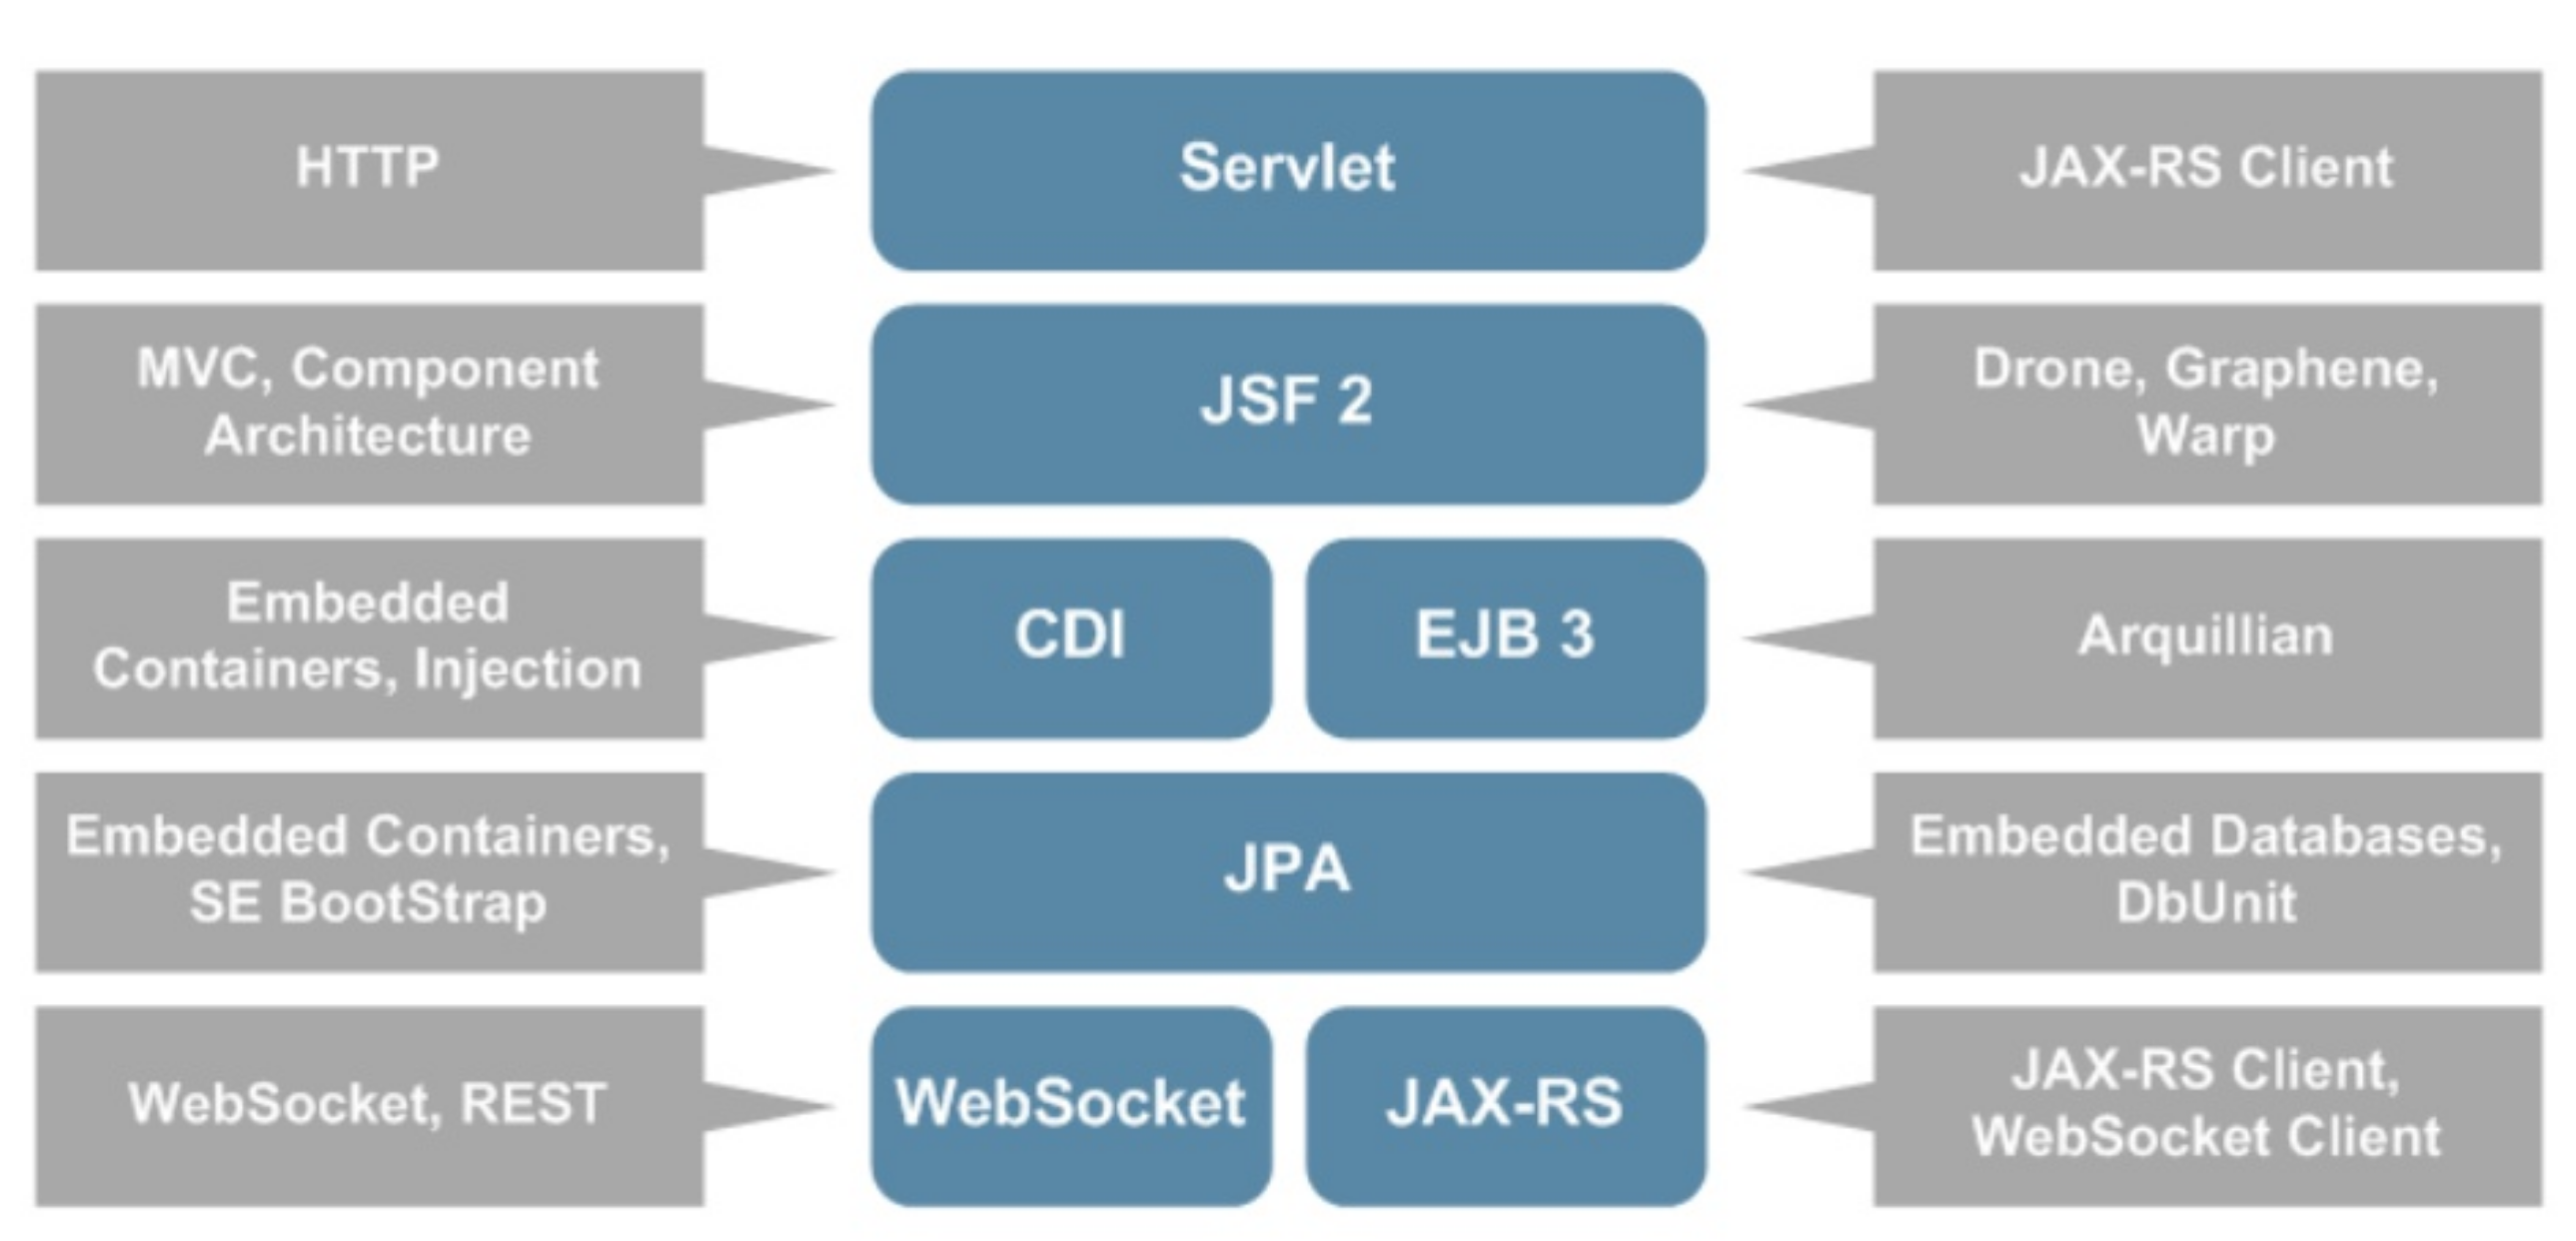
\includegraphics[width=0.8\linewidth]{Images/testingee}
				\caption{Testing Java EE - Créditos: Reza Rahman}
		\end{figure}

\end{frame}


\begin{frame}{Arquillian}

\begin{figure}
	\centering
	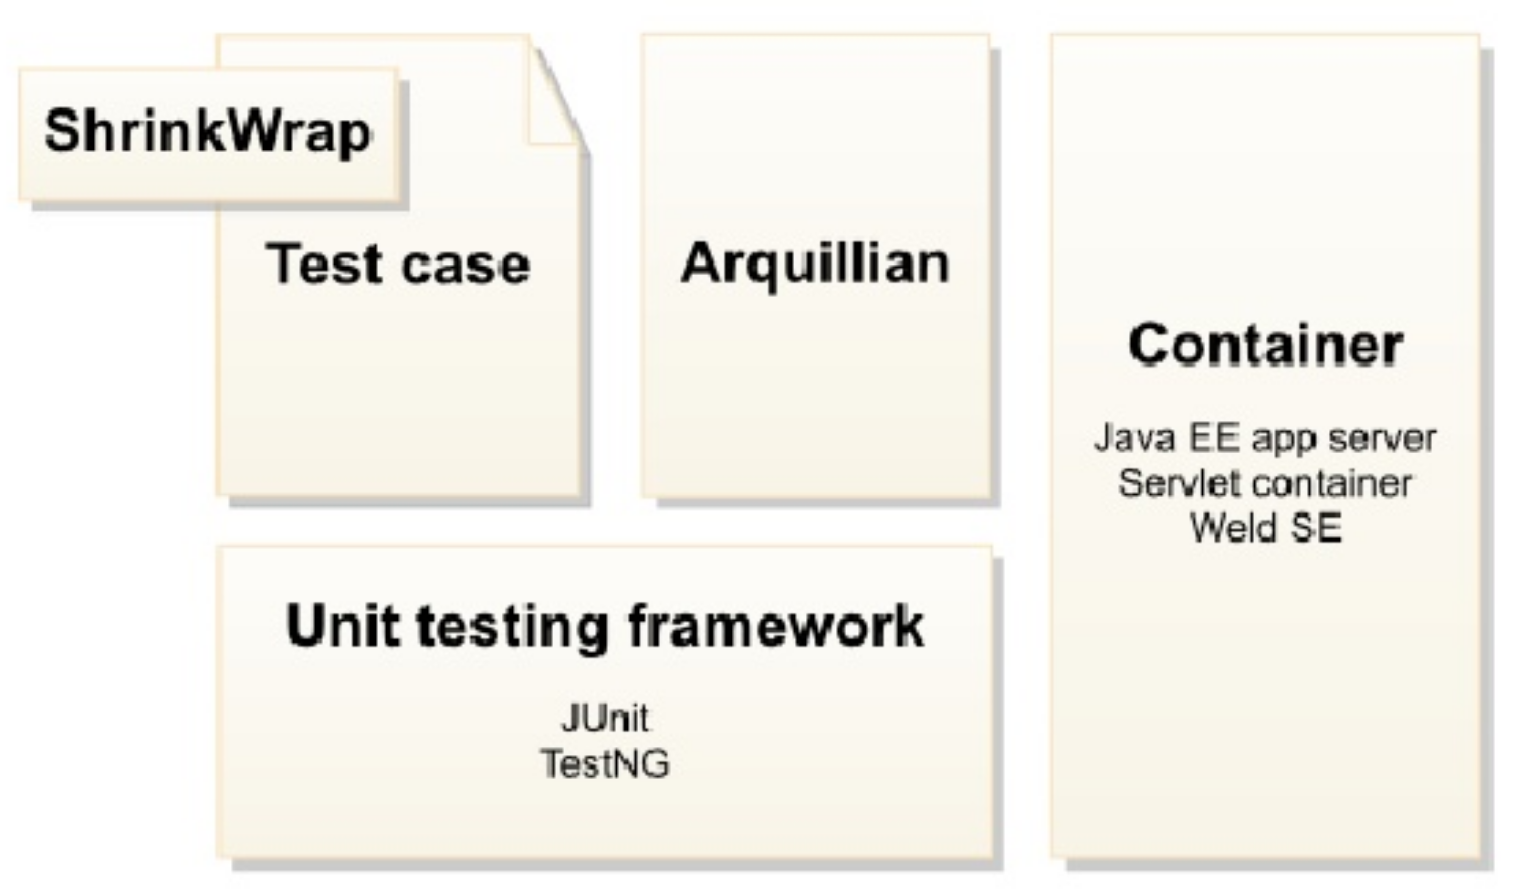
\includegraphics[width=0.8\linewidth]{Images/arquillian}
		\caption{Estructura prueba Arquillian - Créditos: Proyecto Arquillian}
\end{figure}

\end{frame}



\begin{frame}{Arquillian}
\begin{itemize}
	\item Embedded: Misma JVM que el runner
	\item Managed: Contenedor externo, lifecycle con arquillian
	\item Remote: Contenedor externo
\end{itemize}
\end{frame}




\begin{frame}[containsverbatim]{Arquillian - ShrinkWrap}

\begin{lstlisting}[language=Java]
@Deployment
public static WebArchive createDeployment() {
	return ShrinkWrap
		.create(WebArchive.class,
			 "todo-list-servlet-test.war")
		.addClass(ItemServlet.class);
}
\end{lstlisting}
\end{frame}


\begin{frame}{Gracias}
\begin{itemize}
\item vorozco@nabenik.com
\item http://nabenik.com
\end{itemize}
\begin{center}

\includegraphics[width=0.1\linewidth]{Images/cclogo}
\\
This work is licensed under a Creative Commons Attribution-ShareAlike 3.0 Guatemala License.
\end{center}
\end{frame}
\end{document}

